% This LaTeX document needs to be compiled with XeLaTeX.
\documentclass[
  10
]{article}
\usepackage[margin=2cm,includehead=true,includefoot=true,centering,]{geometry}
\usepackage{xcolor}
\usepackage{ucharclasses}
\usepackage{hyperref}
\usepackage{amsmath,amssymb}
\usepackage{amsfonts}
\usepackage[version=4]{mhchem}
\usepackage{stmaryrd}
\usepackage{bbold}
\usepackage{polyglossia}
\usepackage{fontspec}
\usepackage[fontset=none]{ctex}
\usepackage[export]{adjustbox}
\usepackage{tabularx}
\usepackage{booktabs}

\usepackage{setspace}
\setstretch{1.2}

\makeatletter
\@ifundefined{KOMAClassName}{% if non-KOMA class
  \IfFileExists{parskip.sty}{%
    \usepackage{parskip}
  }{% else
    \setlength{\parindent}{0pt}
    \setlength{\parskip}{6pt plus 2pt minus 1pt}}
}{% if KOMA class
  \KOMAoptions{parskip=half}}
\makeatother
\usepackage{longtable,booktabs,array}
\newcounter{none} % for unnumbered tables
\usepackage{calc} % for calculating minipage widths
% Correct order of tables after \paragraph or \subparagraph
\usepackage{etoolbox}
\makeatletter
\patchcmd\longtable{\par}{\if@noskipsec\mbox{}\fi\par}{}{}
\makeatother
% Allow footnotes in longtable head/foot
\IfFileExists{footnotehyper.sty}{\usepackage{footnotehyper}}{\usepackage{footnote}}
\makesavenoteenv{longtable}
\usepackage{graphicx}
\makeatletter
\newsavebox\pandoc@box
\newcommand*\pandocbounded[1]{% scales image to fit in text height/width
  \sbox\pandoc@box{#1}%
  \Gscale@div\@tempa{\textheight}{\dimexpr\ht\pandoc@box+\dp\pandoc@box\relax}%
  \Gscale@div\@tempb{\linewidth}{\wd\pandoc@box}%
  \ifdim\@tempb\p@<\@tempa\p@\let\@tempa\@tempb\fi% select the smaller of both
  \ifdim\@tempa\p@<\p@\scalebox{\@tempa}{\usebox\pandoc@box}%
  \else\usebox{\pandoc@box}%
  \fi%
}
% Set default figure placement to htbp
\def\fps@figure{htbp}
\makeatother
\setlength{\emergencystretch}{3em} % prevent overfull lines
\providecommand{\tightlist}{%
  \setlength{\itemsep}{0pt}\setlength{\parskip}{0pt}}


\hypersetup{colorlinks=true, linkcolor=blue, filecolor=magenta, urlcolor=cyan,}
\urlstyle{same}

\usepackage{colortbl}
\definecolor{table-row-color}{HTML}{999999}
\definecolor{table-rule-color}{HTML}{999999}
%\arrayrulecolor{black!40}
\arrayrulecolor{table-rule-color}     % color of \toprule, \midrule, \bottomrule
\setlength{\aboverulesep}{0pt}
\setlength{\belowrulesep}{0pt}


\setotherlanguages{english}
\IfFontExistsTF{Source Han Serif CN}
{\newfontfamily\chinesefont{Source Han Serif CN}}
{\IfFontExistsTF{Noto Serif CJK SC}
  {\newfontfamily\chinesefont{Noto Serif CJK SC}}
  {\IfFontExistsTF{SimSun}
    {\newfontfamily\chinesefont{SimSun}}
    {\IfFontExistsTF{FangSong}
      {\newfontfamily\chinesefont{FangSong}}
      {\newfontfamily\chinesefont{Arial Unicode MS}}
}}}
\IfFontExistsTF{Times New Roman}
{\newfontfamily\englishfont{Times New Roman}}
{\IfFontExistsTF{Liberation Serif}
  {\newfontfamily\englishfont{Liberation Serif}}
  {\IfFontExistsTF{DejaVu Serif}
    {\newfontfamily\englishfont{DejaVu Serif}}
    {\newfontfamily\englishfont{Arial}}
}}


\author{}
\date{}

\begin{document}


\section{Catalyzer: Sub-millisecond Startup for Serverless Computing
with Initialization-less
Booting}\label{catalyzer-sub-millisecond-startup-for-serverless-computing-with-initialization-less-booting}

Dong \(\mathrm { D u } ^ { \dag \ddag }\) , Tianyi
\(\mathrm { Y u } ^ { \dag \ddag \mathinner { \ S } }\) , Yubin Xia†‡,
Binyu Zang†‡, Guanglu Yan§, Chenggang Qin§, Qixuan
\(\mathrm { W u ^ { \ S } }\) , Haibo Chen†‡

† Shanghai Key Laboratory of Scalable Computing and Systems, Shanghai
Jiao Tong University ‡ Institute of Parallel and Distributed Systems,
Shanghai Jiao Tong University \(\ S\) Ant Financial Services Group

\section{Abstract}\label{abstract}

Serverless computing promises cost-efficiency and elasticity for
high-productive software development. To achieve this, the serverless
sandbox system must address two challenges: strong isolation between
function instances, and low startup latency to ensure user experience.
While strong isolation can be provided by virtualization-based
sandboxes, the initialization of sandbox and application causes
non-negligible startup overhead. Conventional sandbox systems fall short
in low-latency startup due to their application-agnostic nature: they
can only reduce the latency of sandbox initialization through hypervisor
and guest kernel customization, which is inadequate and does not
mitigate the majority of startup overhead.

This paper proposes Catalyzer, a serverless sandbox system design
providing both strong isolation and extremely fast function startup.
Instead of booting from scratch, Catalyzer restores a
virtualization-based function instance from a well-formed checkpoint
image and thereby skips the initialization on the critical path
(init-less). Catalyzer boosts the restore performance by on-demand
recovering both user-level memory state and system state. We also
propose a new OS primitive, sfork (sandbox fork), to further reduce the
startup latency by directly reusing the state of a running sandbox
instance. Fundamentally, Catalyzer removes the initialization cost by
reusing state, which enables general optimizations for diverse
serverless functions. The evaluation shows that Catalyzer reduces
startup latency by orders of magnitude, achieves
\({ < } 1 \mathrm { m s }\) latency in the best case, and significantly
reduces the end-to-end latency for real-world workloads.

Permission to make digital or hard copies of all or part of this work
for personal or classroom use is granted without fee provided that
copies are not made or distributed for profit or commercial advantage
and that copies bear this notice and the full citation on the first
page. Copyrights for components of this work owned by others than the
author(s) must be honored. Abstracting with credit is permitted. To copy
otherwise, or republish, to post on servers or to redistribute to lists,
requires prior specific permission and/or a fee. Request permissions
from permissions@acm.org. ASPLOS '20, March 16--20, 2020, Lausanne,
Switzerland

\(\circledcirc\) 2020 Copyright held by the owner/author(s). Publication
rights licensed to ACM.

ACM ISBN 978-1-4503-7102-5/20/03. . . \$15.00

https://doi.org/10.1145/3373376.3378512

Catalyzer has been adopted by Ant Financial, and we also present lessons
learned from industrial development.

CCS Concepts • Computer systems organization Cloud computing; • Software
and its engineering Operating systems.

Keywords serverless computing; startup latency; checkpoint and restore;
operating system

\section{ACM Reference Format:}\label{acm-reference-format}

Dong Du, Tianyi Yu, Yubin Xia, Binyu Zang, Guanglu Yan, Chenggang Qin,
Qixuan Wu, Haibo Chen. 2020. Catalyzer: Sub-millisecond Startup for
Serverless Computing with Initialization-less Booting. In Proceedings of
the Twenty-Fifth International Conference on Architectural Support for
Programming Languages and Operating Systems (ASPLOS '20), March 16--20,
2020, Lausanne, Switzerland. ACM, New York, NY, USA, 15 pages.
https://doi.org/10.1145/3373376.3378512

\section{1 Introduction}\label{introduction}

Serverless computing, the new trending paradigm in cloud computing,
liberates developers from the distraction of managing servers and has
already been supported by many platforms, including Amazon Lambda
{[}2{]}, IBM Cloud Function {[}1{]}, Microsoft Azure Functions {[}3{]}
and Google Cloud Functions {[}7{]}. In serverless computing, the unit of
computation is a function. When a service request is received, the
serverless platform allocates an ephemeral execution sandbox and
instantiates a user-defined function to handle the request. This
computing model shifts the responsibility of dynamically managing cloud
resources to cloud providers, allowing the developers to focus purely on
their application logic. Besides, cloud providers can manage their
resources more efficiently.

The ephemeral execution sandboxes are typically containers {[}1{]},
virtual machines {[}20, 44{]} or recently proposed lightweight
virtualization designs {[}6, 8, 19, 35, 37, 41, 45{]}. However,
container instances suffer from isolation issues since they share one
kernel, which is error-prone. Virtual machines can achieve better
isolation but are too heavy to run serverless functions. Lightweight
virtualization designs like Google gVisor {[}8{]} and Amazon FireCracker
{[}6{]} achieve high performance, easy resource management and strong
isolation by customizing the host-guest interfaces, e.g., gVisor uses a
process abstraction interface.

\pandocbounded{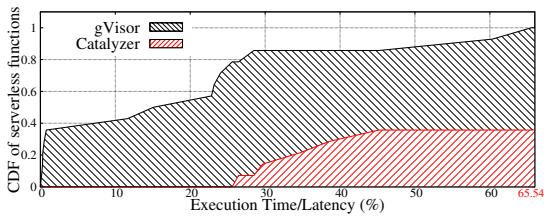
\includegraphics[keepaspectratio,alt={image}]{images/89157301d724057ee3201f62f8ea476f4b69e1933f1276030ff6d68c08e71db8.jpg}}

Figure 1. Distribution of Execution/Overall latency ratio in serverless
computing. The ratio of all functions in gVisor can not even achieve
\(6 5 . 5 4 \%\) . The startup is cold boot.

Executing serverless functions with low latency is critical for user
experience {[}21, 24, 28, 32, 38{]}, and is still a significant
challenge for virtualization-based sandbox design. To explain the
severity, we conduct an end-to-end evaluation on three benchmarks,
DeathStar {[}22{]}, E-business microservices, and image processing
functions, and divide the latency into ``execution'' part and ``boot''
part (§6.4). We calculate the ``Execution/Overall'' ratio of the tested
14 serverless functions, and present the CDF in Figure 1. The ratio of
12 functions (out of 14) in gVisor can not even achieve \(3 0 \%\) ,
indicating that the startup dominates the overall latency. Long startup
latency, especially for virtualization-based sandbox, has become a
significant challenge for serverless platforms.

Existing VM-based sandboxes {[}6, 8, 37{]} reduce the startup latency
through hypervisor customization, e.g., FireCracker can boot a virtual
machine (microVM) and a minimized Linux kernel in 100ms. However, none
of them can reduce the application initialization latency like JVM or
Python interpreter setup time. Our studies on serverless functions
(written by five programming languages) show that most of the startup
latency comes from application initialization (Insight I).

This paper proposes Catalyzer, a general design to boost startup for
serverless computing. The key idea of Catalyzer is to restore an
instance from a well-formed checkpoint image and thereby skip the
initialization on the critical path. The design is based on two
additional insights: First, a serverless function in execution stage
typically accesses only a small fraction of memory and files used in the
initialization stage (Insight II), thus we can on-demand recover both
application state (e.g., data in memory) and system state (e.g., file
handles/descriptors). Second, sandbox instances of the same function
possess almost the same initialized state (Insight III), thus it is
possible to reuse most of the state of running sandboxes to spawn new
ones. Specifically, Catalyzer adopts ondemand recovery of both
user-level and system state. And it proposes a new OS primitive, sfork
(sandbox fork), to further reduce the startup latency by directly
reusing state of a running sandbox instance. Fundamentally, Catalyzer
eliminates the initialization cost by reusing state, which enables
general optimizations on diverse serverless functions.

We have implemented Catalyzer based on gVisor. We measure the
performance with both micro-benchmarks and realworld applications
developed in five programming languages.

The result shows the Catalyzer can achieve \({ < } 1 \mathrm { m s }\)
startup latency on C-hello (best case), and \(< 2 \mathrm { m s }\)
\textless{} to boot Java SPECjbb, \(1 0 0 0 \mathrm { x }\) \textless{}
speedup over baseline gVisor. We also present evaluations on server
machines and share our lessons learned from industrial development at
Ant Financial.

The main contributions of this paper are as follows:

• A detailed analysis of latency overhead on serverless computing (§2).

• A general design of Init-less booting that boosts startup of diverse
serverless applications (§3 and §4).

• An implementation of Catalyzer on a state-of-the-art serverless
sandbox system, Google gVisor (§5).

• An evaluation with micro-benchmarks and real-world serverless
applications proving the efficiency and practicability of Catalyzer
(§6).

• The experience of deploying Catalyzer on real platforms (§6.9).

\section{2 Serverless Function Startup
Breakdown}\label{serverless-function-startup-breakdown}

In this section, we evaluate and analyze the startup latency of
serverless platforms with different system sandboxes (i.e., gVisor,
FireCracker, Hyper Container, and Docker) and different language
runtimes. Based on evaluation and analysis, we present our motivation
that serverless functions should be executed with an initialization-less
approach.

\section{2.1 Background}\label{background}

Serverless Platform. In serverless computing, the developer sends a
function to the serverless platform to execute. We use the term handler
function to represent the target function, which could be written in
different languages. The handler function is compiled offline together
with a wrapper, which does initialization and invokes the handler
function. Wrapped programs (consist of the wrapper and handler function)
execute safely within sandboxes, which can be containers {[}5, 40{]} or
virtual machines (VM) {[}6, 8, 10{]}. There is a gateway program running
on each server as a daemon, which accepts ``invoke function'' requests,
and starts a sandbox with two arguments: a configuration file and a
rootfs containing both the wrapped program and runtime libraries. The
arguments are based on OCI specification {[}12{]} and compatible with
most of the existing serverless platforms.

gVisor Case Study. In this paper, we propose a general optimization to
achieve sub-millisecond startup even for VMbased sandboxes like gVisor.
In the following text, we will take gVisor as an example for analysis,
implementation, and evaluation. For evaluation, we use server machines
(§6.1) to reveal performance improvement in the industrial environment.

On a serverless platform, the first step of invoking a function is to
prepare a sandbox. In the case of gVisor, the sandbox preparation
includes four operations: configuration parsing, virtualization resource
allocation (e.g., VCPUs and guest

\pandocbounded{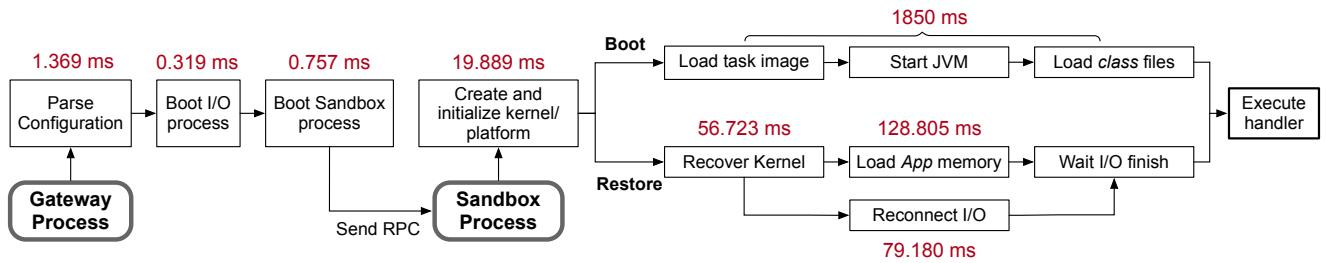
\includegraphics[keepaspectratio,alt={image}]{images/d95f7449ffbf143f74a571c0afa8fab00b3160f503c1090139e58cd9bbda7738.jpg}}

Figure 2. Boot process of gVisor. The numbers are the latency of each
step of Java SPECjbb. The Restore path is the process of restoring a
sandbox from a checkpoint image in gVisor (gVisor-restore).

\pandocbounded{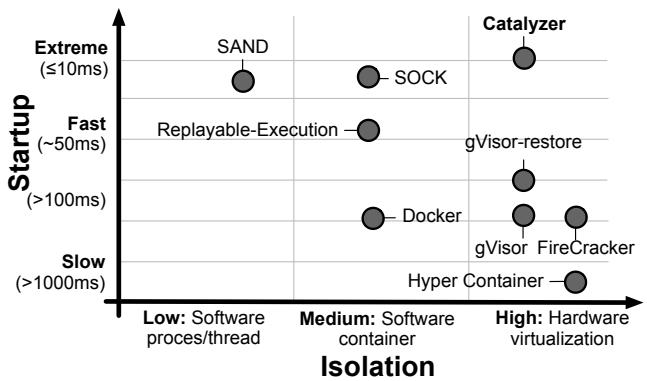
\includegraphics[keepaspectratio,alt={image}]{images/8228a51b1f0f1cf92023dd264858690e9cb537bbffa8f3384bcacf42ebcf6eed.jpg}}

Figure 3. Serverless sandbox design. Catalyzer is the only system that
achieves both high isolation and low startup latency.

memory regions), root file system mounting and guest kernel
initialization (Figure 2). The guest kernel consists of two user
processes: a sandbox process and an I/O process. The sandbox process
sets up the virtualized resource, e.g., the extended page table (EPT)1,
and prepares the guest kernel. The I/O process mounts the root file
system according to the configuration file. Figure 2 shows that sandbox
initialization takes non-negligible time (22.3ms) in gVisor. Since
sandbox initialization depends on function-specific configurations, it
is hard to use techniques like caching {[}31, 40{]} to reduce sandbox
initialization overhead. The critical path of startup refers to the
period from when the ``Gateway process'' got a request until the handler
executed. We use the term offline to represent the non-critical path
operations (e.g., caching).

After sandbox initialization, the sandbox runs the wrapped program
specified in the configuration file. Taking Java as an example, the
wrapped program first starts a JVM to initialize Java runtime (e.g.,
loading class files), then executes the user-provided handler function.
We define the application initialization latency as the period from when
then wrapped program starts until the handler function is ready to run.
As the following evaluation shows, the application initialization
latency dominates the total startup latency.

\section{2.2 A Quantitative Analysis on Startup
Optimizations}\label{a-quantitative-analysis-on-startup-optimizations}

The design space of serverless sandboxes is shown in Figure 3.

Cache-based Optimizations. Many systems adopt the idea of caching for
serverless function startup {[}17, 39, 40{]}. For example, Zygote is a
cache-based design for optimizing latency, which has been used in
Android {[}14{]} to instantiate new Java applications. SOCK {[}40{]}
leverages the Zygote idea for serverless computing. By creating a cache
of pre-warmed Python interpreters, functions can be launched with an
interpreter that has already loaded the necessary libraries, thus
achieve high startup performance. SAND {[}17{]} allows instances of the
same application function to share the sandbox which contains the
function codes and its libraries. However, there are two reasons that
caching is far from ideal. First, a single machine is capable of running
thousands of serverless functions, so caching all the functions in
memory will introduce high resource overhead. Caching policies are also
hard to be determined in the real-world. Second, caching does not help
with the tail latency, which is dominated by the ``cold boot'' in most
cases.

Optimizations on Sandbox Initialization. Besides caching sandbox systems
also optimize their initialization through customization. For example,
SOCK {[}40{]} proposes a lean container, which is a customized container
design for serverless computing, to mitigate the overhead of sandbox
initialization. Compared with container-based approaches, VM-based
sandboxes {[}6, 8, 10{]} provide stronger isolation and also introduce
more costs to sandbox initialization. Researchers have proposed numerous
lightweight virtualization techniques {[}6, 19, 26, 36, 37{]} to solve
performance and resource utilization issues {[}18, 23, 25, 29{]} in
traditional heavy-weight virtualization systems. These proposals have
already stimulated significant interest in serverless computing industry
(e.g., Google's gVisor {[}8{]} and Amazon's FireCracker {[}6{]}).

Further, the lightweight virtualization techniques adopt various ways to
optimize startup latency: by customizing guest kernels {[}26, 36{]},
customizing hypervisors {[}19, 37{]} or a combination of the two {[}6,
8{]}. For instance, FireCracker {[}6{]} can boot a virtual machine
(microVM) and a minimized Linux

\pandocbounded{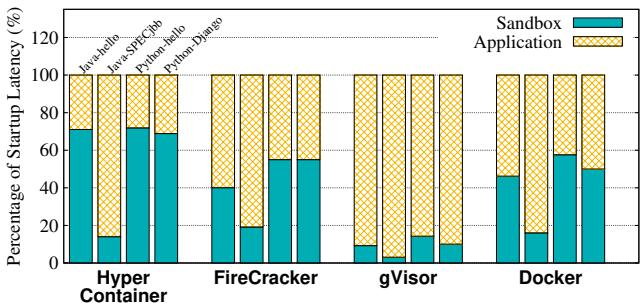
\includegraphics[keepaspectratio,alt={image}]{images/0fda6754aad3d502ad54da07aa835fb23cdc22bc31430d68e00926352a1c103c.jpg}}

Figure 4. Startup latency distribution. Application initialization costs
dominate in complex applications like Java SPECjbb, while sandbox
initialization costs are significant for lightweight applications like
Python Hello.

kernel in \(1 0 0 \mathrm { m s }\) . Although different in design and
implementation, today's virtualization-based sandboxes have one common
limitation: they can not mitigate the application initialization latency
like JVM or Python interpreter.

To understand the latency overhead (including sandbox and application
initialization), we evaluate the startup latency of four widely used
sandboxes (i.e., gVisor, FireCracker, Hyper Container, and Docker) with
different workloads, and present the latency distribution in Figure 4.
The evaluation uses the sandbox runtime directly and does not count the
cost of container management. The settings are the same as described in
\(\ S 6 . 1\) .

We highlight several interesting findings from the evaluation. First,
much of the latency overhead comes from application initialization.
Second, compared with C language (142ms startup latency in gVisor), the
startup latency is much higher for high-level languages like Java and
Python. The main reason is that high-level languages usually need to
initialize a language runtime (e.g., JVM) before loading application
codes. Third, sandbox initialization is stable for different workloads
and dominates the latency overhead for simple functions like Python
Hello.

The evaluation shows that much of the startup latency comes from
application initialization instead of sandbox. However, none of the
existing virtualization-based sandboxes can reduce the application
initialization latency caused by JVM or Python interpreter.

\pandocbounded{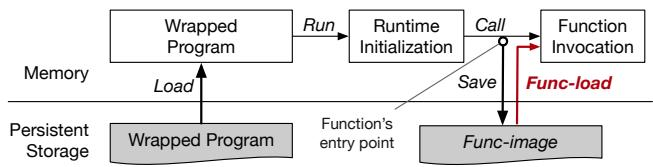
\includegraphics[keepaspectratio,alt={image}]{images/9fa93cbeda06c2bd78bb991fdd02c542150c78825e881e7080c51f09aefab51d.jpg}}

Figure 5. Init-less booting.

Checkpoint/Restore-based Optimizations. Checkpoint/restore (C/R) is a
technique to save state of a running sandbox into a checkpoint image.
The saved state includes both application state (in the sandbox) and
sandbox state (e.g., the

\pandocbounded{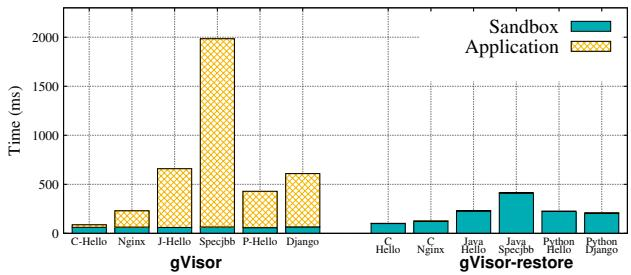
\includegraphics[keepaspectratio,alt={image}]{images/896c52a21da9643400eaf579d03ef12ec9194f6f4a4927394f3d2169dca5a23b.jpg}}

Figure 6. Startup latency of gVisor and gVisor-restore. gVisorrestore
adopts C/R to eliminate the application initialization cost, but still
has high startup (restore) latency.

hypervisor). Then, the sandbox can be restored from the image and run
seamlessly. Replayable Execution {[}43{]} leverages C/R techniques to
mitigate the application initialization cost, but only apply to
container-based systems. Compared with other C/R systems, Replayable
optimizes memory loading using an on-demand approach for boosting
startup latency. However, our evaluation shows virtualization-based
sandboxes incur high overhead to recover system state during the
restore, which is omitted by the prior art.

The major benefit of C/R is that it can transform the application
initialization costs into the sandbox restore costs (initless). We
generalize the idea as Init-less booting, shown in Figure 5. First, a
func-image (short for function image) is generated offline, which saves
initialized state of a serverless function (Offline initialization). The
func-image could be saved to both local or remote storage, and a
serverless platform needs to fetch a func-image first. After that, the
platform can re-use the state saved in the func-image to boost the
function startup (func-load).

Challenges. C/R (checkpoint/restore) techniques re-use serialized state
(mostly application state) of a process to diminish application
initialization cost, but rely on re-do operations to recover system
state (i.e., in-kernel state like the opened files). A re-do operation
recovers the state of a checkpointed instance and is necessary for
correctness and compatibility. For example, a C/R system will re-do
``open()'' operations to re-open files that are opened in a checkpointed
process. However, re-do operations introduce performance overhead,
especially for virtualization-based sandboxes.

To analyze the performance effect, we implement a C/Rbased init-less
booting system on gVisor, called gVisor-restore, using gVisor-provided
checkpoint and restore {[}4{]} mechanism. We add a new syscall in gVisor
to trap at the entry point of serverless functions. We use the term,
func-entry point, to indicate the entry point of a serverless function,
which is either specified by developers or at the default location: the
point right before the wrapped program invoking the handler function.
The syscall is invoked by the func-entry point annotation and will block
until checkpoint operation begins.

We evaluate the startup latency of gVisor-restore using different
applications, and compare with unmodified gVisor. We use the sandbox
runtime directly (i.e., runsc for gVisor) to exclude container
management cost. As the result (Figure 6) shows, gVisor-restore
successfully eliminates the application initialization overhead and
achieves \(2 \mathrm { X } ^ { - 5 \mathrm { X } }\) speedup over
gVisor. However, the startup latency is still high (400ms for a Java
SPECjbb application and \({ > } 1 0 0 \mathrm { m s }\) in other cases).
Figure 2 suggests that gVisor-restore spends
\(1 3 5 . 9 \mathrm { m s }\) on guest kernel recovery, which can be
classified into ``Recover Kernel'' and ``Reconnect I/O'' in the figure.
The ``Recover Kernel'' means recovering non-I/O system state, e.g.,
thread information, while I/O reconnection is for recovering I/O system
state, e.g., re-open a ``suppose opened'' file. For reusable state
(``App memory'' in the figure), gVisor C/R mechanism compresses the
saved data to reduce the storage overhead, and needs to decompress,
deserialize, and load the data into memory on the restore critical path,
costing 128.8ms for a SPECjbb application. During the restore process in
SPECjbb case, gVisor recovers more than 37,838 objects (e.g.,
threads/tasks, mounts, sessionLists, timers, and etc.) in guest kernel
and loads 200MB memory data.

Prior container-based C/R systems {[}43{]} have exploited on-demand
paging to boost application state recovery, but still recover all the
system state in the critical path.

\section{2.3 Overview}\label{overview}

Our evaluation and analysis motivate us to propose Catalyzer, an
init-less booting design for virtualization-based sandboxes, which is
equipped with novel techniques to overcome the high latency on the
restore process.

\pandocbounded{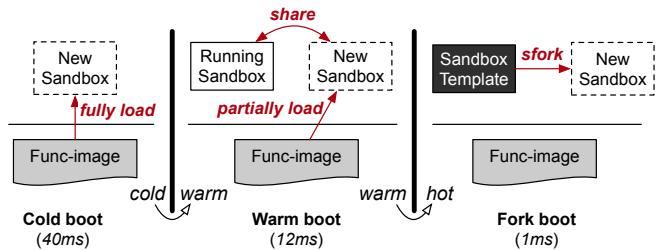
\includegraphics[keepaspectratio,alt={image}]{images/ef1d485c18f5fb10bd2c68fef425bbdaabd4c8df6420d0c060f5c9dca6867708.jpg}}

Figure 7. Overview of Catalyzer. Catalyzer combines C/R and sandbox fork
to boost both cold boot and hot boot.

As shown in Figure 7, Catalyzer defines three kinds of booting: cold
boot, warm boot, and fork boot. Precisely, cold boot means that the
platform must create a sandbox instance from func-image through restore.
Warm boot means there are running instances for the requested function;
thus, Catalyzer can boost the restore by sharing in-memory state of
running instances. Fork boot in Catalyzer needs a dedicated sandbox
template, a sandbox contains the initialized state, to skip the
initialization. Fork boot is a hot-boot mechanism {[}11, 40{]}---a
platform that knows a function may be invoked soon and prepares the
running environment for the function. The

significant contribution is that fork boot is scalable to boot any
number of instances from a single template, while prior hot boot can
only serve limited instances (depending on the cache size).

Catalyzer adopts a hybrid approach combining C/R-based init-less booting
and a new OS primitive to implement the cold, warm, and fork boot. Since
a serverless function in the execution stage typically accesses only a
small fraction of both memory and files used in the initialization
stage, Catalyzer introduces on-demand restore for cold and warm boot to
optimize the recovery of both application and system state (§3). In
addition, Catalyzer proposes a new OS primitive, sfork (sandbox fork),
to reduce the startup latency in fork boot by directly reusing the state
of a template sandbox (§4). Fork boot can achieve faster startup than
the warm boot, but also introduces more memory overhead; thus, fork boot
is more suitable for frequently invoked (hot) functions.

\section{3 On-demand Restore}\label{on-demand-restore}

The performance overhead of restore comes from two parts. First, the
application and system state need to be uncompressed, deserialized (only
metadata) and loaded into memory. Second, re-do operations are necessary
to recover system state, including multi-threaded contexts,
virtualization sandbox and I/O connections.

As shown in Figure 8-a, Catalyzer accelerates restore by splitting the
process into three parts: offline preparation, critical path restore,
and on-demand recovery. The preparation work, like uncompression and
deserialization, is mostly performed offline in the checkpoint stage.
The loading of application state and recovering of I/O-related system
state are delayed with on-demand paging and I/O re-connection. Thus,
Catalyzer only performs minimized work on the critical path, i.e.,
recovering non-I/O system state.

Specifically, Catalyzer proposes four techniques. First, overlay memory
is a new memory abstraction that allows Catalyzer to directly map a
func-image into memory, boosting application state loading (for cold
boot). Sandboxes running the same function can share a ``base memory
mapping'', further omitting file mapping cost (for warm boot). Second,
separated state recovery decouples deserialization from system state
recovery on the critical path. Third, on-demand I/O reconnection delays
I/O state recovery. Last, virtualization sandbox Zygote provides
generalized virtualization sandboxes that are function-independent and
can be used to reduce sandbox construction overhead.

\section{3.1 Overlay Memory}\label{overlay-memory}

The overlay memory is a design for on-demand application state loading
through copy-on-write of file-based mmap. As shown in Figure 8-b, the
design allows a ``base memory mapping'' to be shared among sandboxes
running the same

\pandocbounded{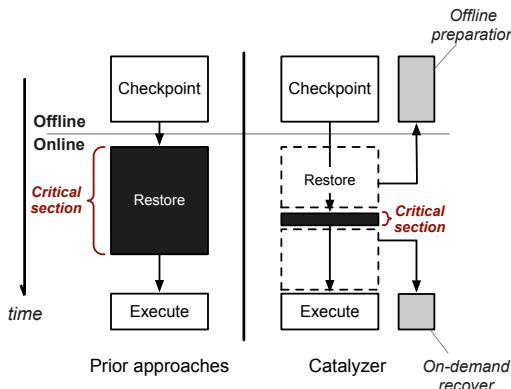
\includegraphics[keepaspectratio,alt={image}]{images/09a98ccbebad1e63428996a52f98674d30bab169cfd61ffee9895a184f38fa88.jpg}}

\begin{enumerate}
\def\labelenumi{(\alph{enumi})}
\tightlist
\item
  Comparison.
\end{enumerate}

\pandocbounded{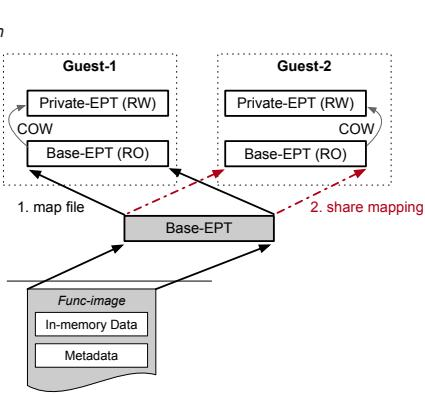
\includegraphics[keepaspectratio,alt={image}]{images/37e78c61f648cebc84980300b13a6e05ef022367f47b4e887c85e7045c173bbf.jpg}}

\begin{enumerate}
\def\labelenumi{(\alph{enumi})}
\setcounter{enumi}{1}
\tightlist
\item
  Overlay memory.
\end{enumerate}

\pandocbounded{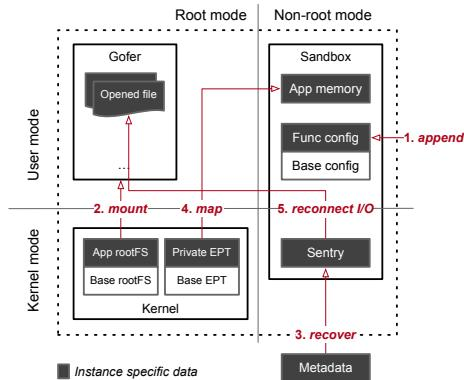
\includegraphics[keepaspectratio,alt={image}]{images/bdfda5a2ae412253c138d494bb41c58f0fe2067db003ba79f5096a310919575a.jpg}}

\begin{enumerate}
\def\labelenumi{(\alph{enumi})}
\setcounter{enumi}{2}
\tightlist
\item
  Operational flow.
\end{enumerate}

Figure 8. On-demand restore. (a) Compared with prior approaches,
Catalyzer leverages offline preparation and on-demand recovery to
eliminate most of the work on the critical path. (b) Overlay memory
allows a func-image to be directly mapped into memory to construct the
Base-EPT, and the Base-EPT can also be shared among different instances
through copy-on-write. (c) The operational flow shows how a gVisor
sandbox is instantiated using on-demand restore.

function, and relies on memory copy-on-write to ensure privacy.

Overlay memory uses a well-formed func-image for direct mapping, which
contains uncompressed and page-aligned application state. During a cold
boot, Catalyzer loads application state by directly mapping the
func-image into memory (map-file operation). Catalyzer maintains two
layered EPTs for each sandbox. The upper one is called Private-EPT, and
the lower one is Base-EPT. Private-EPT is private to each sandbox, while
Base-EPT is shared and read-only. During a warm boot, Catalyzer directly
maps the Base-EPT for the new sandbox with the share-mapping operation.
The main benefit comes from the avoidance of costly file loading.

The platform constructs the hardware EPT by merging entries from the
Private-EPT with the Base-EPT, i.e., using the entries of Private-EPT if
the entries are valid, otherwise using the entries of Base-EPT. The
construction is efficient and triggerd by hardware. Base-EPT is
read-only thus can be inherited by new sandboxes through mmap, while the
Private-EPT is established using copy-on-write when an EPT violation
happens on the Base-EPT.

\section{3.2 Separated State Recovery}\label{separated-state-recovery}

C/R relies on metadata of system state (represented by objects in the
sandbox) for re-do operation, which is serialized before saving into
checkpoint images and deserialized during the restore. The system state
includes all guest OS internal state, e.g., the thread list and timers.
However, such process is non-trivial for sandboxes implemented by
high-level languages (e.g., Golang for gVisor), as the language
abstraction hides the arrangement of state data. Even with the help of
serialization tools such as Protobuf {[}16{]}, metadata objects have to
be processed one-by-one to recover, which can cause huge

overhead when the number of objects is large (e.g., 37,838 objects are
recovered for SPECjbb application in gVisor-restore, consuming
\(> 5 0 \mathrm { m s }\) ).

\begin{quote}
Catalyzer proposes separated state recovery to overcome the challenge,
by decoupling deserialization from state recovery. During offline
preparation, Catalyzer saves partially deserialized metadata objects
into func-images. Specifically, Catalyzer first re-organizes the
discrete in-memory objects into continuous memory; thus they can be
mapped back to memory through mmap operation instead of one-by-one
deserialization. Then, Catalyzer zeros pointers in objects with
placeholders, and records all (pointer) reference relationships in a
relation table, which stores a map from offsets of pointers to offsets
of pointer values. The metadata objects and the relation table together
constitute the partially deserialized objects. The partially means that
Catalyzer needs to deserialize pointers during runtime using the
relation table.
\end{quote}

With the func-image, Catalyzer accomplishes state recovery in two
stages: loading the partially deserialized objects from a func-image
(stage-1), reconstructing the object relationships (e.g., pointer
relation) and recovering system state in parallel (stage-2). First,
objects as well as the saved relation table will be mapped to the
sandbox's memory with overlay memory. Second, the object reference
relationships are re-established by replacing all placeholders with real
pointers through the relation table, and non-I/O system state are
established on the critical path. Since each update is independent, this
stage can be carried out in parallel. The design does not depend on a
specific memory layout, which is better for portability so that a
func-image can run on different machines.

\section{3.3 On-demand I/O
Reconnection}\label{on-demand-io-reconnection}

The numerous I/O operations performed in restore (e.g., opening files)
add high latency on the critical path. Inspired

by our insight that many of the I/O-related state (e.g., files) will not
be used after restore, Catalyzer adopts an on-demand I/O reconnection
design. For example, a previously opened file ``/home/user/hello.txt''
may only be accessed for specific requests. Those unused I/O connections
can not be eliminated even with a proper point in the checkpoint,
because existing serverless functions are usually running with language
runtime (e.g., JVM) and third-party libraries, in which the developers
have no idea whether they will access some rarely used connections.

Thus, we can re-establish the connections lazily---only reestablish when
the connections are used. To achieve this, I/O reconnection is performed
asynchronously on the restore critical path, and the sandbox guest
kernel maintains the I/O connection status, i.e., a file descriptor will
be passed to functions but tagged as not re-opened yet in the guest
kernel.

We observe that for a specific function, the I/O connections that are
immediately used after booting are mostly deterministic. Thus, we
introduce an I/O cache mechanism to further mitigate the latency of I/O
reconnection. The I/O connection operations performed during cold boot
are saved in cache, which are used by Catalyzer to guide a sandbox (in
warm boot) to establish these connections on the critical path.
Specifically, the cache stores the file paths and the operations on the
path, so Catalyzer can use the information as a hint to re-connect these
I/O first. For I/O connections missed in the cache (i.e., the
non-deterministic connections), Catalyzer will use the on-demand
strategy to establish the needed I/O connections.

\section{3.4 Virtualization Sandbox
Zygote}\label{virtualization-sandbox-zygote}

On the restore critical path, a sandbox is constructed before
application state loading and system state recovery. Challenges of
reducing sandbox construction latency lie in two factors: first, sandbox
construction depends on functionspecific information (e.g., the path of
rootfs), thus techniques like caching do not help; second, a sandbox is
tightly coupled with system resources that are not directly re-usable
(e.g., namespace and hardware virtualization resources).

Catalyzer proposes a Virtualization Sandbox Zygote design that separates
the function-dependent configuration from a general sandbox (Sandbox
Zygote) and leverages a cache of Zygotes to mitigate sandbox
construction overhead. A Zygote is a generalized virtualization sandbox
used to generate a function-specific sandbox during the restore. As
described in Figure 2, a sandbox is constructed with a configuration
file and a rootfs. Catalyzer proposes a base configuration and a base
rootfs, which separate out function-specific details. Catalyzer caches a
Zygote by parsing the base configuration file, allocating virtualization
resources (e.g., VCPU) and mounting the base rootfs. Upon function
invocation, Catalyzer specializes a sandbox from a Zygote by importing
function-specific

binaries/libraries, and appending the function-specific configuration in
the Zygote. Virtualization Zygotes can be used in both cold boot and
warm boot in Catalyzer.

\section{3.5 Putting All Together}\label{putting-all-together}

The three elements, overlay memory, separated state, and I/O
connections, are all included in the func-image. The workflow of cold
boot and warm boot is shown in Figure 8-c.~First, function-specific
configuration and its func-image (in ``App rootFS'') is passed to a
Zygote to specialize a sandbox. Second, the function-specific rootfs
indicated by the configuration is mounted for the sandbox. Then, the
sandbox recovers system state using separated state recovery. After
that, Catalyzer maps the Base-EPT 's memory to the gVisor process as
read-only for warm boot, in which copy-on-write is used to preserve the
privacy of the sandbox's memory. For cold boot, Catalyzer needs to
establish the Base-EPT first by mapping the func-image into memory. At
last, the guest kernel asynchronously recovers I/O connections, and I/O
cache assists the process for warm boot.

\section{4 sfork: Sandbox fork}\label{sfork-sandbox-fork}

Based on our Insight III, Catalyzer proposes a new OS primitive, sfork
(sandbox fork), to further reduce the startup latency by reusing the
state of a running ``template sandbox'' directly. The term, ``template
sandbox'', means a special sandbox for a specific function that has no
information about user requests; thus, it can be leveraged to
instantiate sandboxes to serve requests. The basic workflow is shown in
Figure 9-a. First, a template sandbox is generated through template
initialization, containing clean system state at the func-entry point;
then, when a request of the function arrives, the template sandbox will
sfork itself to reuse the initialized state directly. The state here
includes both user state (application and runtime) and guest kernel
state.

Challenges. An intuitive choice is to use the traditional fork to
implement sfork. However, it is challenging to keep system state
consistent by using fork only. First, most OS kernels (e.g., Linux) can
only support single-thread fork, which means the information of
multi-threading will be lost after forking. Second, fork is not suitable
for sandbox creation, during which a child process will inherit its
parent's shared memory mappings, file descriptors and other system state
that are not supposed to be shared between sandboxes. Third, fork will
clone all the user state in memory, some of which may depend on system
state that have been changed. For example, given a common case where the
template sandbox issues getpid syscall and uses the return value to name
a variable during initialization, the PID is changed in the forked
sandbox, but the variable is not, leading to undefined behavior.

The clone syscall provides more flexibility with many options, but is
still not sufficient. One major limitation is the

\pandocbounded{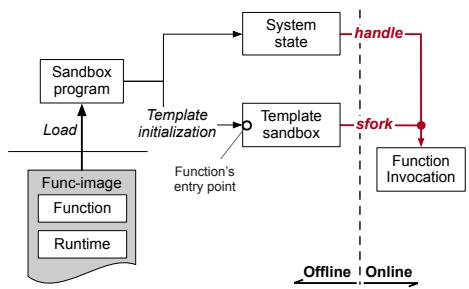
\includegraphics[keepaspectratio,alt={image}]{images/e7b2431a4d0f4e5dd65bc555bb413047bbb565e5cb86b54e9afa06dbda544023.jpg}}

\begin{enumerate}
\def\labelenumi{(\alph{enumi})}
\tightlist
\item
  Overview of sandbox fork.
\end{enumerate}

\pandocbounded{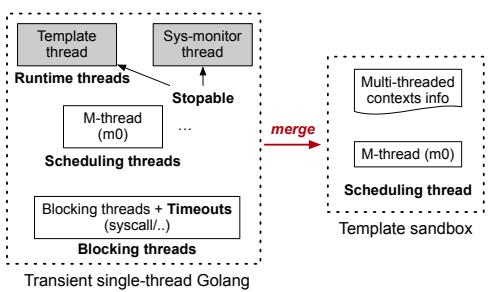
\includegraphics[keepaspectratio,alt={image}]{images/883cfb76a68135479e39415ffc29470bbf9b52476287290a5ab5948d8343e92d.jpg}}

\begin{enumerate}
\def\labelenumi{(\alph{enumi})}
\setcounter{enumi}{1}
\tightlist
\item
  Transient single-thread for Golang.
\end{enumerate}

\pandocbounded{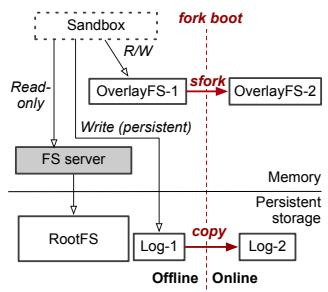
\includegraphics[keepaspectratio,alt={image}]{images/f19d4ce790aa02be4efbafd2b40449781c3203bb9639e1c52662c411375846b1.jpg}}

\begin{enumerate}
\def\labelenumi{(\alph{enumi})}
\setcounter{enumi}{2}
\tightlist
\item
  Stateless overlayFS.
\end{enumerate}

Figure 9. Catalyzer with sandbox fork. (a) Catalyzer can sfork a new
instance from a template sandbox generated offline. (b) The transient
single-thread mechanism can support multi-threading fork by temporarily
merge a multi-threaded program into a single thread. (c) Stateless
overlay rootfs achieves efficient handling for file descriptors and
files.

handling of shared memory (mapped with MAP\_SHARED flag). If a child
sandbox inherits the shared memory, it will violate the isolation
between parent and child sandboxes; if not, it may change the semantics
of MAP\_SHARED.

Template Initialization. To overcome the challenges, Catalyzer relies on
user-space handling of most inconsistent state and only introduces
minimal kernel modifications. We classify syscalls into three groups,
denied, handled and allowed. The allowed and handled syscalls are listed
in Table 1. The handled syscalls require user-space logic to fix related
system state after sfork for consistency explicitly. For example, clone
creates a new thread context for a sandbox, and the multi-threaded
contexts should be recovered after sfork (Challenge-1). The denied
syscalls are removed from the sandbox since they may lead to
non-deterministic system state modification. We illustrate how Catalyzer
keeps the multi-threaded contexts and reuses inherited file descriptors
(Challenge-2) after sfork with two novel techniques, transient
single-thread and stateless overlay rootFS. The only modification to the
kernel is adding a new flag, CoW flag, for shared memory mapping. We
take advantage of Linux container technologies (USER and PID namespaces)
to maintain system state like user id and process id consistent after
sfork (Challenge-3).

\section{4.1 Multi-threading Fork}\label{multi-threading-fork}

Sandboxes implemented using Golang (e.g., gVisor) are naturally
multi-threaded, because the Golang runtime uses multiple threads for
garbage collection and other background works. Specifically, threads in
Golang can be classified into three categories: runtime threads,
scheduling threads, and blocking threads (Figure 9-b). The runtime
threads are responsible for providing runtime functionalities like
garbage collection and preemption. They are long-running and transparent
to the developers. The scheduling threads (M-threads in Figure 9-b)
implement the co-routine mechanism in Golang (i.e., Go routine). When a
Go routine switches to the blocked state (e.g., executing blocking
system calls like accept), Golang runtime will dedicate an OS thread to
the Go routine.

Catalyzer proposes a transient single-thread mechanism to support
multi-threaded sandbox fork. With the mechanism, a multi-threaded
program can temporarily merge all the threads into a single thread
(i.e., the transient singlethread), which can be expanded to a
multi-threaded one after sfork. The process is shown in Figure 9-b.
First, we modify the Golang runtime in Catalyzer to support stoppable
runtime threads. When the runtime threads are notified to enter the
transient single-thread state, they will save the thread contexts in the
memory and terminate themselves. Then, the number of scheduling threads
can be configured to one through Golang runtime. In addition, we add a
time-out in all blocking threads, and the threads will check whether
they should terminate for entering the transient single-thread state
when the time-out is triggered. Finally, the Golang program will only
keep the m0 thread in the transient singlethread state, and expand to
multiple threads again after sfork. Our modification is only used for
template sandbox generation, and will not affect program behaviors after
sfork.

\section{4.2 Stateless Overlay RootFS}\label{stateless-overlay-rootfs}

A sforked sandbox will inherit file descriptors and file systems of the
template sandbox, which should be handled after sfork. Inspired by
existing overlayFS design {[}13{]} and the ephemeral nature of
serverless functions {[}27, 28{]}, Catalyzer employs stateless overlay
rootFS technique to achieve zerocost handling for file descriptors and
the rootFS. The idea is to put all the modification on the rootFS into
the memory, which can be automatically cloned during sfork using
copy-on-write (Figure 9-c).

Specifically, each sandbox uses two layers of file systems. The upper
layer is the in-memory overlayFS, which is private to a sandbox and
allows both read and write operations. The overlayFS is backed by an FS
server (per-function) which manages the real rootFS. A sandbox cannot
directly access the persistent storage for security reasons; thus, it
relies on the (read-only) file descriptors received from the FS server
to access the rootFS. During sfork, besides the cloned overlayFS, the
file descriptors owned by the template sandbox are still

{\def\LTcaptype{none} % do not increment counter
\begin{longtable}[]{@{}|l|l|l|@{}}
\toprule\noalign{}
\endhead
\bottomrule\noalign{}
\endlastfoot
\hline
Categories & Operators & Operators \\
\hline
Proc & Transient single-thread, Namespace & capget, clone, getpid,
gettid, arch\_prctl, prctl, rt\_sigaction, rt\_sigprocmask,
rt\_sigreturn, seccomp, sigaltstack, sched\_getaffinity \\
\hline
VFS (FS/Net) & Read-only FD & poll, ioctl, memfd\_create, ftruncate,
mount, pivot\_root, umount, epoll\_create1, epollCtl, epoll\_pwait,
eventfd2, fcntl, chdir, close, dup, dup2, lseek, openat \\
\hline
File (Storage) & Stateless overlayFS & newstat, newstatat, mkdirat,
write, read, readlinkat, preadd4 \\
\hline
Network & Reconnect & sendmsg, shutdown, recvmsg, getsockopt, listen,
accept \\
\hline
Mem & Handled by sfork & mmap, munmap \\
\hline
Misc & Namespace & setgid, setuid, get(e)gid, get(e)uid, getrandom,
nanosleep, futex, getgroups, clock\_gettime, getrlimit, setsid \\
\hline
\end{longtable}
}

Table 1. Syscall classification used in Catalyzer for sfork. Non-bold
font means allowed but not handled syscalls, while bold font is for
handled syscalls. The allowed syscalls can run as normal syscalls.
Handlers are only used for handled syscalls.

\pandocbounded{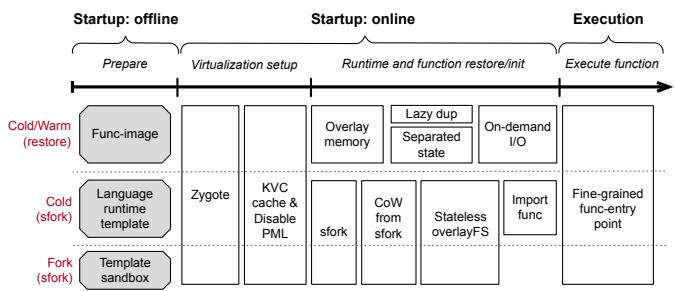
\includegraphics[keepaspectratio,alt={image}]{images/11f0b639eecfc937d672a87d3e16f319e8e5f8a24e7ad60e7ffe1479ee58ae24.jpg}}

Figure 10. Techniques/Optimizations used in Catalyzer for different
kinds of boot. Besides techniques introduced in §3 and \(\ S 4\) ,
Catalyzer has other optimizations like the fine-grained funcentry point
to further reduce startup latency.

valid in the child sandbox since they are read-only and will not violate
the isolation guarantee.

Our industrial development lessons show that persistent storage is still
required for serverless functions in some cases, e.g., writing logs.
Catalyzer allows the FS server to grant some file descriptors of the log
files (with the read/write permission) to sandboxes. Overall, the
majority of files are sforked with low latency, and only a small number
of persistent files are copied for functionalities.

\section{4.3 Language Runtime Template for Cold
Boot}\label{language-runtime-template-for-cold-boot}

Although the on-demand restore can provide promising cold boot
performance, it relies on a well-formed func-image containing
uncompressed data (larger image size). Thus, we propose another choice
for the cold boot, using sfork with language runtime template, which is
a template sandbox for functions written by the same language. A
language runtime template initializes the environment of the wrapped
program (e.g., JVM in Java), and will load a real function to serve
requests on demand. Such a sandbox should be instantiated differently in
different languages, e.g., loading libraries in C or loading Class files
in Java. For instance, a single Java runtime template is sufficient to
boost our internal functions as most of the functions are written in
Java.

\section{5 Implementation}\label{implementation}

Catalyzer is implemented based on gVisor, with 2017 LoC modification in
gVisor and 732 LoC modification in Golang runtime for sfork, and 5000
lines of Golang modification to support the Init-less booting and
optimizations. In addition, we extend our platform with a kernel module
(about 300 lines of C) and a user-level manager program (500 lines of
Golang).

Besides the techniques proposed in the design, Catalyzer leverages other
optimizations to further reduce startup latency, e.g., the fine-grained
func-entry point (§6.7). We present an overall view on how these
techniques and optimizations are used in Catalyzer for different boots,
as shown in Figure 10. The details will be explained in \(\ S 6 . 7\) .

Func-image Compilation. The offline func-image compilation is performed
by the following steps: 1) The func-entry point provided by the user is
inserted into the wrapper program as an annotation; 2) The func-entry
point annotation is transferred to a system call invocation
(Gen-Func-Image in Catalyzer) in the wrapper program. For example, in C,
the annotation is replaced by a call to ``syscall()'' of libC; in Java,
the wrapper program uses JNI codes to invoke the syscall. Any invocation
of the syscall is taken as ``the program reaches the func-entry point'',
and triggers Catalyzer to save the state; 3) The wrapper program starts
to run, and traps into the gVisor kernel when it reaches the func-entry
point; 4) The current program state, including in-memory data, system
metadata and the I/O information is saved into the generated func-image.
Most of the image compilation process is automated. Catalyzer uses the
func-image for cold boot, and re-uses in-memory state of existing
running instances for warm and fork boot.

Generality. Although we choose to implement Catalyzer on gVisor/Golang,
the design is general, and most of the techniques are also applicable to
other lightweight virtualization systems. For example, FireCracker
{[}6{]} needs more than 100ms to boot a guest kernel, which can be
optimized safely with the on-demand restore. The four techniques in
on-demand restore (e.g., overlay memory) only depend on

hardware virtualization extensions like Intel EPT or AMD NPT. Moreover,
the transient single-thread of sfork is also general and can be used in
other Golang-based virtualization systems (e.g., Google novm {[}9{]}).

\section{6 Evaluation}\label{evaluation}

In the evaluation, we try to answer the following questions:

• Question-1: How does Catalyzer improve the startup performance of
diverse applications? (§6.2)

• Question-2: How does each technique in Catalyzer improve the startup
performance individually? (§6.3)

• Question-3: How does Catalyzer reduce the latency of end-to-end
serverless functions? (§6.4)

• Question-4: How does Catalyzer reduce memory usage of a serverless
platform? (§6.5)

• Question-5: How is the scalability of Catalyzer when there are 1000
running instances? (§6.6)

• Question-6: How does Catalyzer achieve near 1ms latency through
optimizations? (§6.7)

• Question-7: Will Catalyzer introduce new security issues? (§6.8)

• Question-8: What can we learn from industrial development? (§6.9)

\section{6.1 Evaluation Environment}\label{evaluation-environment}

We use an x86-64 machine (the experimental machine) with an 8-core Intel
i7-7700 CPU, 32GB memory and Samsung 512GB SSD, to evaluate
microbenchmarks and performance breakdown. The OS is Ubuntu 16.04 with
Linux kernel 4.17.3. In addition, we use a server machine from Ant
Financial, with 96 cores (@ 2.50\,GHz) and
256GB memory for end-toend latency and scalability evaluation. We
compare several serverless platforms, including gVisor (commit
\#56fa562), FireCracker (commit \#28f44b3) using the official minimized
kernel, Docker runc (commit \#bbb17ef) and Hyper Container (commit
\#565496c).

\section{6.2 Application Startup
Latency}\label{application-startup-latency}

We evaluate the startup latency of Catalyzer with diverse applications
written by different programming languages to answer the first question.

Methodology. We compare cold boot (Catalyzer-restore), warm boot
(Catalyzer-Zygote) and fork boot (Catalyzer-sfork) with Docker
container, Hyper container, gVisor, gVisor-restore, and FireCracker. We
chose applications written by five languages: C, Java, Python, Ruby, and
Node.js, which are widely supported in existing serverless platforms.
For each language, we test two workloads. One is ``helloworld'' which
represents the minimal application, and the other is a real application.
We do not evaluate Ruby on FireCracker since the official kernel
provided by FireCracker does not support Ruby yet.

Table 2. Cold boot with Java runtime templates.

{\def\LTcaptype{none} % do not increment counter
\begin{longtable}[]{@{}|l|l|l|l|@{}}
\toprule\noalign{}
\endhead
\bottomrule\noalign{}
\endlastfoot
\hline
Systems & Native & gVisor & Java template \\
\hline
Cold boot (ms) & 89.4 & 659.1 & 29.3 \\
\hline
\end{longtable}
}

The C application is a widely used web server, Nginx (version 1.11.3).
The latency is evaluated as the time from the ``nginx'' command to the
start of its main function. SPECjbb2015 is a widely used benchmark to
evaluate the Java server business scenarios. We evaluate the time
between the ``java'' command and the entry of BackendAgent. Django is
used for Python application and Sinatra for Ruby applications, which are
both web frameworks/libraries for applications. For Node.js, we use a
web server as the tested application.

Results. Figure 11 shows the result. Catalyzer achieves the best
performance in all the applications. Specifically, Catalyzersfork can
boost startup latency of a serverless function to even less than 1ms
(0.97ms in C-hello). Catalyzer-Zygote can boot a serverless function
using 5ms for C, 14ms for Java, 9ms for Python, 12ms for Ruby, and 9ms
for Node.js applications. Catalyzer-restore usually needs extra 30ms
over Catalyzer-Zygote to initialize the sandbox and map funcimage into
memory. The results also reveal the improvement of Catalyzer is general
for diverse applications, from the simple C-hello to Java-SPECjbb.

Language Runtime Templates. The sfork primitive is proposed for hot boot
in most cases. However, with the language runtime templates design
(§4.3), sfork can provide a general template for diverse functions
written by the same language (to achieve fast cold boot for lightweight
functions). As shown in Table 2, we evaluate the latency of booting a
lightweight Java-based function, using a JVM runtime template. The
latency is about 20ms longer than Catalyzersfork, but still
\(3 0 \mathrm { x }\) faster than baseline gVisor. Moreover, Java
template sandbox can even boost the startup latency better than the
native \(3 . 0 \mathrm { x }\) and \(3 . 7 \mathrm { x }\) faster). The
major overhead of Catalyzer-sfork is caused by loading Java class files
of requested functions.

\section{6.3 Improvement Breakdown}\label{improvement-breakdown}

We evaluate the optimization of the three techniques used in Catalyzer
(cold boot). The baseline is the gVisor-restore. We evaluate the startup
latency of two applications, Python Django and Java SPECjbb with four
configurations, the baseline (gVisor-restore), Catalyzer without
separated loading and lazy reconnection, Catalyzer without lazy
reconnection, and Catalyzer.

As shown in Figure 12, overlay memory can reduce 261ms of latency for
Java SPECjbb compared with the gVisor-restore. Separated object loading
reduces the kernel loading latency by 6.3x for Python Django, and
\(7 . 0 \mathrm { x }\) for Java SPECjbb, Lazy

\pandocbounded{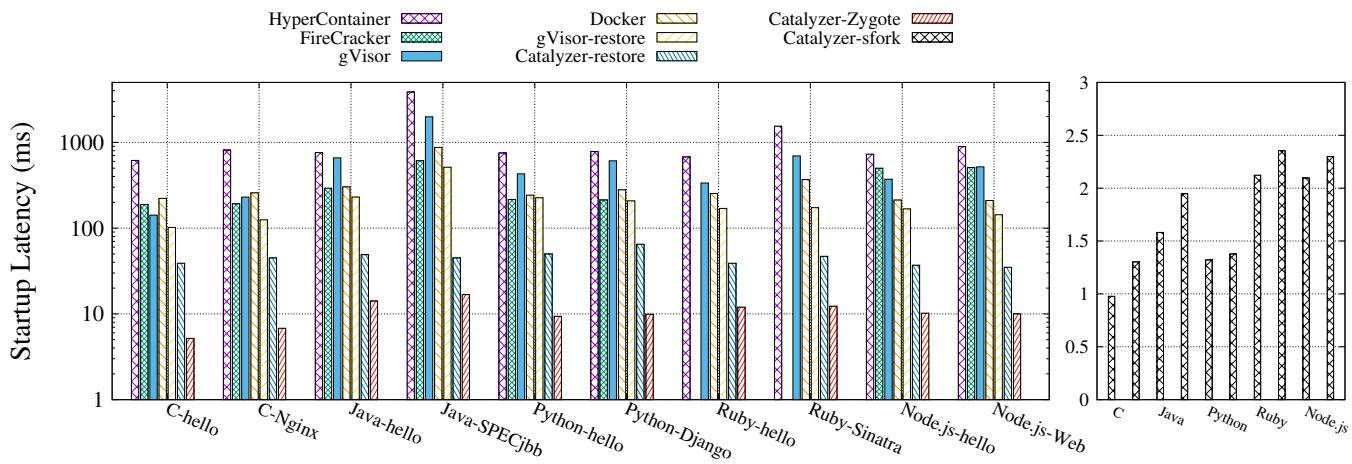
\includegraphics[keepaspectratio,alt={image}]{images/eb7f755b975e5e4f9a4e74b39b0c82517565f9dbe99cfc855de2e6d79502c91f.jpg}}

Figure 11. Startup latency of Catalyzer compared with other systems. The
test cases for Catalyzer-sfork (right part) are the same.

\pandocbounded{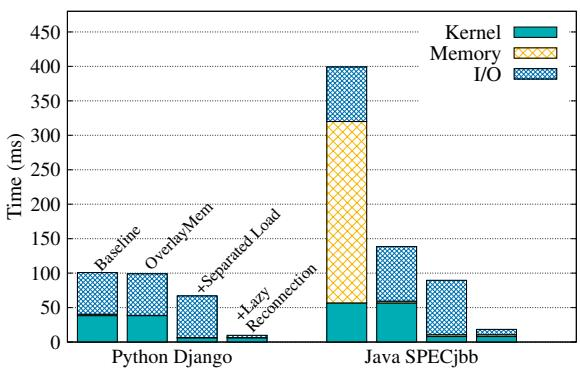
\includegraphics[keepaspectratio,alt={image}]{images/5f62973159daf055e47fd2f4f5bf01c628289c5a08147c2d69afc35be1c38dd4.jpg}}

Figure 12. Breakdown of Catalyzer (cold boot) on gVisor.

I/O reconnection reduces \(> 5 7 \mathrm { m s }\) of latency on I/O
reconnec-\textgreater tion in both two applications, namely,
\(1 8 \mathrm { x }\) improvement. The result shows that applications
with small memory footprint can benefit more from separated object
loading and lazy I/O reconnection, while overlay memory contributes most
of the optimization for applications with large memory footprint.

\section{6.4 End-to-End Evaluation}\label{end-to-end-evaluation}

We present three end-to-end tests to show how Catalyzer can reduce
latency for real-world serverless functions. In each case, we present
the startup latency (Boot) and the execution latency (Execution). We
compare three systems, gVisor, Catalyzer-sfork (fork boot) and
Catalyzer-restore (cold boot).

DeathStar Social Network Microservices. DeathStar {[}22{]} is an
open-source microservice benchmark. We port five microservices in
DeathStar social network benchmark to our serverless platform.
Specifically, all microservice invocations in selected microservices are
replaced by stub functions to be compatible with the platform.

The results are shown in Figure 13-a. DeathStar represents real-world
lightweight serverless functions. All the selected

functions are written in \(\mathrm { C } { + } { + }\) , and have
\(< 2 . 5 \mathrm { m s }\) execution \textless time in all the cases,
as shown in the figure. For these functions, Catalyzer can significantly
reduce the overall latency by boosting startup
\(3 5 \mathrm { x } \mathrm { - } 6 7 \mathrm { x }\) using sfork).

Image Processing Application. Image processing can be implemented as
serverless functions and has been deployed in existing platforms
{[}17{]}. We use Python Pillow {[}15{]}, a Python imaging library to
implement five major tasks for image processing. Specifically, the
Pillow applications receive images, process them (i.e.,
enhance/filter/roll/splitmerge/- transpose the images), and then return
the processed results.

As shown in Figure 13-b, the execution time of the five functions are
\(1 0 0 { - } 2 0 0 \mathrm { m s }\) . The major cost is from reading
the input images. Although the execution time is much longer than
DeathStar, the startup latency still dominates the overall latency
\(\left( > 5 0 0 \mathrm { m s } \right)\) . Overall, Catalyzer can
reduce the end-to-\textgreater end latency by
\(4 . 1 \mathrm { X } ^ { - 6 . 5 \mathrm { X } }\) in fork boot, and
\(3 . 6 \mathrm { X } ^ { - 4 . 3 \mathrm { X } }\) in cold boot,
compared with the baseline.

E-commerce Functions. We evaluate four E-commerce serverless functions
written in Java: purchase, advertising, report generation, and discount
applying. The execution time of these services varies from hundreds of
milliseconds (report generation) to more than one second (purchase). We
compare the Boot and Execution latency of them running in gVisor and
Catalyzer.

The results are shown in Figure 13-c.~In baseline gVisor, booting of the
four Java applications contributes to \(3 4 \% - 8 8 \%\) of their
end-to-end latency. In Catalyzer, the number drops below \(5 \%\) ,
which is a significant improvement over existing systems and is
acceptable in most server service scenarios.

\section{6.5 Memory Usage Evaluation}\label{memory-usage-evaluation}

On-demand Paging. Figure 14 compares memory usages of the DeathStar
composePost function in gVisor and Catalyzer (with sfork) under
concurrent running sandboxes (from 1

\pandocbounded{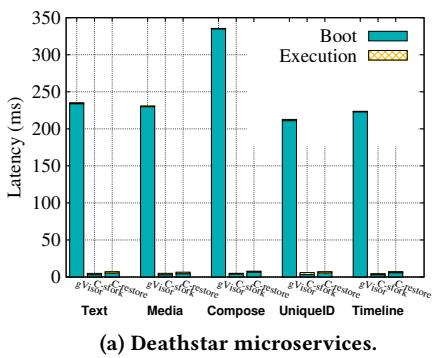
\includegraphics[keepaspectratio,alt={image}]{images/060915cf5c3801063931aac3c942646725df134d9fc029c924ea57357745f449.jpg}}

\pandocbounded{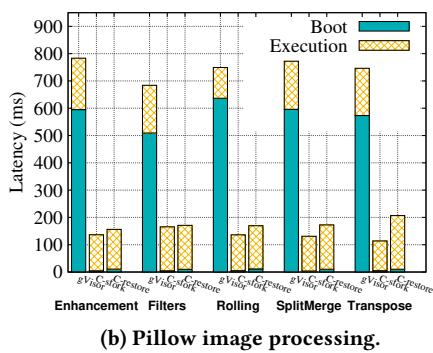
\includegraphics[keepaspectratio,alt={image}]{images/02ca13c54929d60cfe9bc999009ad8cb6f16433b10287e1cd42820ea513e5fbb.jpg}}

\pandocbounded{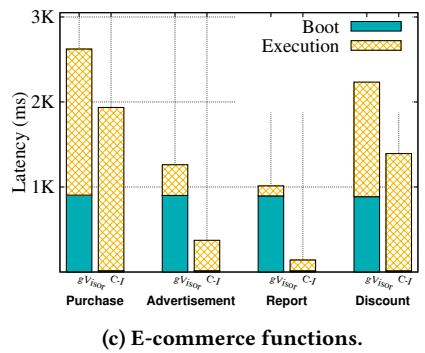
\includegraphics[keepaspectratio,alt={image}]{images/e47696e3dc8466b5939bcae14f9188ab6475208dbbef3d67585907fe83486b12.jpg}}

Figure 13. End-to-end evaluation. C-sfork means fork boot of Catalyzer,
C-restore means cold boot of Catalyzer, and C-I means Catalyzer on the
server machine.

\pandocbounded{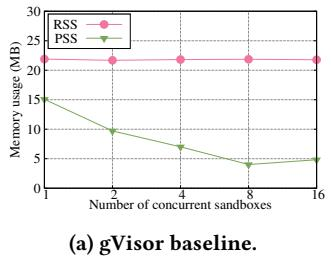
\includegraphics[keepaspectratio,alt={image}]{images/19c97f2c1754385d5e64fd5f2de3434914a355f40a62c66abef9433720412080.jpg}}

\pandocbounded{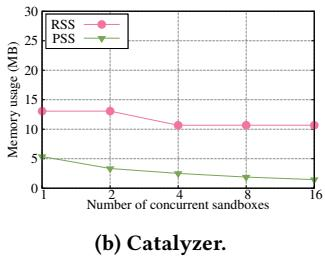
\includegraphics[keepaspectratio,alt={image}]{images/58190f206cfe0abc4f6bb80d8af4a42276941e9c7bffa4c9b1739a4b48fab1dc.jpg}}

Figure 14. Memory usages in the DeathStar.

Table 3. Memory costs in Catalyzer for warm boot.

{\def\LTcaptype{none} % do not increment counter
\begin{longtable}[]{@{}|l|l|l|l|@{}}
\toprule\noalign{}
\endhead
\bottomrule\noalign{}
\endlastfoot
\hline
Applications & Metadata Objects & I/O Cache & All \\
\hline
C-Nginx & 165.5KB & 370B & 165.9KB \\
\hline
Java-SPECjbb & 680.6KB & 2.4KB & 683.0KB \\
\hline
Python-Django & 289.3KB & 1.2KB & 290.5KB \\
\hline
Ruby-Sinatra & 349.2KB & 1.5KB & 350.8KB \\
\hline
NodeJS-Web & 302.1KB & 472B & 302.6KB \\
\hline
\end{longtable}
}

instance to 16). We use resident set size (RSS) and the proportional set
size (PSS) to represent the memory usage. RSS is the total memory used
by a process, while PSS is composed by the private memory of that
process plus the proportion of shared memory with other processes. Each
point in the figure shows the average value of memory usages over all
running sandboxes. A comparison of the two figures shows that Catalyzer
achieves lower RSS and private memory usages (indicated by PSS)
comparing to gVisor.

Memory Costs of Catalyzer. Memory costs of warm boot in Catalyzer are
acceptable. We have observed that many metadata objects will be copied
into Private-EPT, which incurs memory overhead. We present the costs of
metadata objects and I/O caches in Table 3, which are negligible. For
most applications, Catalyzer needs \({ \leq } 2 . 4 \mathrm { K B }\)
for I/O caches, 165--680KB for metadata objects. Notably, the overhead
is per serverless function (not per serverless instance), making the
cost \(\leq 6 8 3 \mathrm { K B }\) overall) acceptable for most cases.
sfork will introduce more memory overheads, e.g., a SPECjbb template
sandbox can cost \({ > } 2 0 0 M \mathrm { B }\) memory.

\pandocbounded{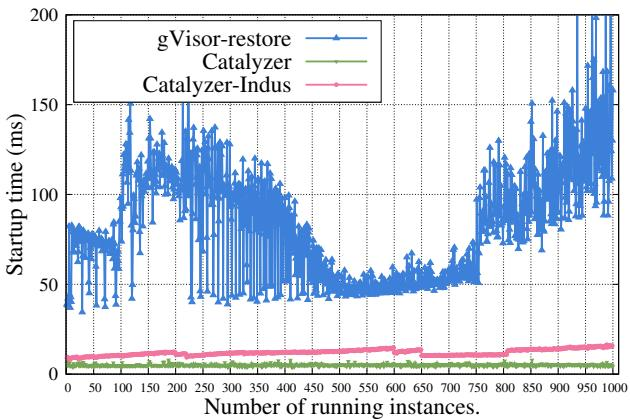
\includegraphics[keepaspectratio,alt={image}]{images/dc0d9b30ecebf3e5452ad8b13f2a6e2819176419b4296576866fdaa00831f7ad.jpg}}

Figure 15. Startup latency as the instance number increases.
Catalyzer-Indus means results from the server machine.

\section{6.6 Concurrent Running}\label{concurrent-running}

One appealing feature of serverless computing is auto-scaling. Hence,
having many serverless instances running simultaneously in a machine is
a common case. We evaluate the startup time of Catalyzer when there are
concurrently running instances.

We use the DeathStar text service as the test function, which handles a
request and hangs a while before exit, for evaluation. As shown in
Figure 15, we evaluate the booting latency with
\(n \left( 0 { - } 1 0 0 0 \right)\) running instances. We compared
Catalyzer with gVisor-restore and only considered the restore latency of
gVisor-restore (without ``create'' sandbox latency). Overall, the
startup latency in Catalyzer is less than \(1 0 \mathrm { m s }\) on
both the experimental machine and the server machine.

\section{6.7 Optimizations}\label{optimizations}

Customized func-entry point. Carefully choosing the funcentry point
location, e.g., moving it after the in-function preparation logic, can
further improve the performance of serverless functions. Using the
optimization, the developers should put the func-entry point in their
function code. The developers should be careful to ensure privacy and
security. Further, a platform can even warm up some dependencies of a

\pandocbounded{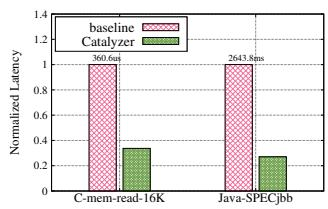
\includegraphics[keepaspectratio,alt={image}]{images/0092e4f63473ff81adfca8ec8d5cfff62af259f0b992960835d0c171972ee167.jpg}}

\begin{enumerate}
\def\labelenumi{(\alph{enumi})}
\tightlist
\item
  Fine-grained func-entry point.
\end{enumerate}

\pandocbounded{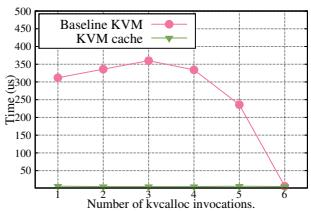
\includegraphics[keepaspectratio,alt={image}]{images/12a9ed1f8db0d4a3183e38e1bca0c3a129ffa7c94bd8ef3c6554a94b5f5f1f59.jpg}}

\begin{enumerate}
\def\labelenumi{(\alph{enumi})}
\setcounter{enumi}{1}
\tightlist
\item
  KVM allocation cache.
\end{enumerate}

\pandocbounded{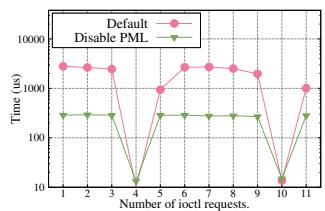
\includegraphics[keepaspectratio,alt={image}]{images/539432357dcf693650d5c01082be021b8407dd46f83b68946b4ca068f914083a.jpg}}

\begin{enumerate}
\def\labelenumi{(\alph{enumi})}
\setcounter{enumi}{2}
\tightlist
\item
  Latency of set\_memory\_region.
\end{enumerate}

\pandocbounded{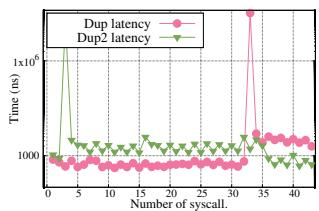
\includegraphics[keepaspectratio,alt={image}]{images/1020056c8496c78a993a335a36145a94b458d0e48bda7e7dcb84af435d160e99.jpg}}

\begin{enumerate}
\def\labelenumi{(\alph{enumi})}
\setcounter{enumi}{3}
\tightlist
\item
  Latency of dup/dup2 syscall.
\end{enumerate}

Figure 16. Optimizations in Catalyzer. Figure (a) shows finegrained
func-entry point can reduce the execution latency by 3x. From Figure
(b), adding a cache in KVM can reduce the latency of kvcalloc. Figure
(c) shows the latency of \_ \_ ioctl set memory region in KVM and
disabling PML achieves 10x shorter latency. Figure (d) shows the latency
of dup syscall during boot. The burst one takes about 30 ms for the
syscall.

function with user-provided requests as training and use the warmed
state as func-image (user-guided pre-initialization). Thus, the time of
application-dependent preparation work can be mitigated.

We use a case in Java SPECjbb and a memory reading C program (as
microbenchmark) for evaluation. The C program will allocate a memory
region to read and write. We move the func-entry point after memory
allocation. For SPECjbb, we move the func-entry point after its
initialization logic. As shown in Figure 16-a, the execution latency is
reduced by 3x for both cases.

Optimizing KVM. Page modification logging (PML), which is a
virtualization feature to monitor changes made to guest physical pages,
is enabled by default in current KVM. If the guest does not need the
feature, it has to be disabled, or it will introduce high latency when
adding a new memory region, as shown in Figure 16-c.~A trick we employed
is to disable PML by default for both the baseline and our systems,
which reduces 5--8ms of latency for setting KVM memory regions.

In addition, KVM uses to allocate memory rekvcallocsource for VM
management, which can incur 1.6ms overhead, as shown in Figure 16-b. To
mitigate the cost, we add a dedicated cache in KVM to boost the
allocations, which can reduce the overhead to \(< 5 0 \mathrm { u s }\)
in most cases.

High Tail Latency System Calls. System call invocation on the host
kernel can incur high latency. For example, dup and dup2 take \(\le 1\,\mathrm{ms}\) to
30ms to finish (Figure 16-d). The burst

latency comes from rare cases in the kernel. For example, the kernel may
expand the fdtable when the table size is not enough, which causes long
latency. Thus, we use a lazy dup, in which the Gofer process first
returns an available fd and duplicate a new one for itself, to mitigate
the overhead. This optimization is implemented in the Gofer process for
on-demand I/O reconnection, which contributes to 10--20ms improvement.

\section{6.8 Security Analysis}\label{security-analysis}

Catalyzer shares a ``base mapping'' among instances. Since the ``base
mapping'' only contains user requests independent state, the sharing
will not leak data or create new cache side channels. A possible issue
is the violation of ASLR (Address Space Layout Randomization), which can
be mitigated by periodically updating func-images and template sandboxes
or adopting previous techniques {[}33, 34{]} to re-randomize the layout
of address space during sfork.

\section{6.9 Lessons Learned from Industrial
Development}\label{lessons-learned-from-industrial-development}

Heavyweight-functions. Prior work focuses on lightweight languages for
serverless functions, e.g., Python. However, a trend is that more
functions are directly ported from welltested service code written in
Java. Thus, a system to boost the startup latency of functions wrapped
with a heavyweight language runtime is necessary. Recent work {[}43{]}
on boosting Java-based serverless functions also confirms the necessity.

Sustainable Hot Boot. Most of existing serverless platforms use function
caches to provide ``hot boot''. However, the benefits of caching depend
on its policies and caching can not help reduce tail latency, which is
dominated by the ``cache miss boot'' in most cases. Our fork boot using
sfork guarantees a sustainable hot boot for functions.

The usage of sfork still depends on workloads and platforms. For private
serverless platforms, it is reasonable to assign different priorities to
different functions; therefore, the platform can use sfork to boot high
priority functions. For a public platform, some hints from the
developers are necessary to improve the boot switching policies to
better leverage the efficiency of fork boot.

\section{7 Related Work}\label{related-work}

Besides the systems mentioned in Section 2, there are other systems
{[}30, 42, 43{]} that have tried to leverage the checkpoint/restore
mechanism for instantiation. Flash cloning {[}42{]} uses a reference
image which contains the memory snapshot of a pre-initialized OS and
application environment. SnowFlock {[}30{]} provides a fast VM
instantiation scheme using VM fork, allowing a virtual machine to fork a
new instance to handle requests. The two systems target traditional
virtual machines, and thus still have high latency, e.g., VM cloning
operation in SnowFlock introduces near second latency. Replayable
Execution {[}43{]} identifies two

execution phases of FaaS applications and extends the checkpoint/restore
mechanism with on-demand paging to achieve 54ms JVM boot. Catalyzer has
two key distinctions. First, on-demand paging is not sufficient in
virtualization-based sandboxes, as system state recovery occupies
prominent overheads. Thus, Catalyzer adopts the on-demand recovery also
for system state. Second, Catalyzer further proposes sfork primitive and
achieves 1.5ms--2ms latency for Java functions.

Unikernels like Mirage {[}36{]} and OSv {[}26{]} can achieve faster
startup than traditional VM by minimizing and customizing the guest OS
for applications and removing the isolation between kernel and
applications. LightVM {[}37{]} can achieve \({ < } 1 0 \mathrm { m s }\)
Unikernel booting by optimizing Xen and minimizing the guest
environment. Catalyzer uses a different idea to boost startup by
skipping the initialization, which is much more efficient and suitable
for serverless. Besides, we believe that Catalyzer can also be applied
to Unikernels.

\section{8 Conclusion}\label{conclusion}

This paper presents Catalyzer, a general design for serverless to boost
the function startup by eliminating the initialization phase with
on-demand restore and sfork. We implement the design based on gVisor,
and the evaluation shows that Catalyzer can significantly reduce the
latency overhead of diverse serverless applications.

\section{Acknowledgments}\label{acknowledgments}

We thank our shepherd Mike Swift and the anonymous reviewers for their
insightful comments. This work is supported in part by the National Key
Research \& Development Program (No.~2016YFB1000104), and the National
Natural Science Foundation of China (No.~61972244, 61925206), the
HighTech Support Program from Shanghai Committee of Science and
Technology (No.~19511121100), and the Program of Shanghai
Academic/Technology Research Leader (No.19XD1401700). Yubin Xia
(xiayubin@sjtu.edu.cn) is the corresponding author.

\section{References}\label{references}

{[}1{]} {[}n.d.{]}. Apache OpenWhisk is a serverless, open source cloud
platform. http://openwhisk.apache.org/. Referenced December 2018.

{[}2{]} {[}n.d.{]}. AWS Lambda - Serverless Compute.
https://aws.amazon.com/ lambda/. Referenced December 2018.

{[}3{]} {[}n.d.{]}. Azure Functions Serverless Architecture.
https://azure. microsoft.com/en-us/services/functions/. Referenced
December 2018.

{[}4{]} {[}n.d.{]}. Checkpoint/Restore in gVisor.
https://gvisor.dev/docs/user\_ guide/checkpoint\_restore/. Referenced
July 2019.

{[}5{]} {[}n.d.{]}. The Docker Containerization Platform.
https://www.docker. com/. Referenced December 2018.

{[}6{]} {[}n.d.{]}. Firecracker. https://firecracker-microvm.github.io/.
Referenced December 2018.

{[}7{]} {[}n.d.{]}. Google Cloud Function.
https://cloud.google.com/functions/. Referenced December 2018.

{[}8{]} {[}n.d.{]}. Google gVisor: Container Runtime Sandbox.
https://github. com/google/gvisor. Referenced December 2018.

{[}9{]} {[}n.d.{]}. google/novm: Experimental KVM-based VMM for
containers, written in Go. https://github.com/google/novm. Referenced
Jan 2020.

{[}10{]} {[}n.d.{]}. Hyper - Make VM run like Container.
https://hypercontainer.io/. Referenced December 2018.

{[}11{]} {[}n.d.{]}. Keeping Functions Warm - How To Fix AWS Lambda Cold
Start Issue. https://serverless.com/blog/keep-your-lambdas-warm/.
Referenced July 2019.

{[}12{]} {[}n.d.{]}. OCI Runtime Specification.
https://github.com/opencontainers/ runtime-spec. Referenced December
2018.

{[}13{]} {[}n.d.{]}. Overlay Filesystem. https://www.kernel.org/doc/
Documentation/filesystems/overlayfs.txt. Referenced July 2019.

{[}14{]} {[}n.d.{]}. Overview of memory management \textbar{} Android
Developers. https:
//developer.android.com/topic/performance/memory-overview. Referenced
December 2018.

{[}15{]} {[}n.d.{]}. Pillow: the friendly PIL fork.
https://python-pillow.org/. Referenced December 2018.

{[}16{]} {[}n.d.{]}. Protocol Buffers Google Developers.
https://developers.google. com/protocol-buffers/. Referenced July 2019.

{[}17{]} Istemi Ekin Akkus, Ruichuan Chen, Ivica Rimac, Manuel Stein,
Klaus Satzke, Andre Beck, Paarijaat Aditya, and Volker Hilt. 2018.
\{SAND\}: Towards High-Performance Serverless Computing. In 2018
\{USENIX\} Annual Technical Conference (\{USENIX\} \{ATC\} 18).
923--935.

{[}18{]} Nadav Amit and Michael Wei. 2018. The Design and Implementation
of Hyperupcalls. In 2018 USENIX Annual Technical Conference (USENIX ATC
18). USENIX Association, Boston, MA, 97--112. https://www.
usenix.org/conference/atc18/presentation/amit

{[}19{]} Adam Belay, Andrea Bittau, Ali José Mashtizadeh, David Terei,
David Mazières, and Christos Kozyrakis. 2012. Dune: Safe User-level
Access to Privileged CPU Features.. In Osdi, Vol. 12. 335--348.

{[}20{]} Fabrice Bellard. 2005. QEMU, a fast and portable dynamic
translator.. In USENIX Annual Technical Conference, FREENIX Track, Vol.
41. 46.

{[}21{]} Sol Boucher, Anuj Kalia, David G. Andersen, and Michael
Kaminsky. 2018. Putting the ``Micro'' Back in Microservice. In 2018
USENIX Annual Technical Conference (USENIX ATC 18). USENIX Association,
Boston, MA, 645--650.
https://www.usenix.org/conference/atc18/presentation/ boucher

{[}22{]} Yu Gan, Yanqi Zhang, Dailun Cheng, Ankitha Shetty, Priyal
Rathi, Nayan Katarki, Ariana Bruno, Justin Hu, Brian Ritchken, Brendon
Jackson, et al.~2019. An Open-Source Benchmark Suite for Microservices
and Their Hardware-Software Implications for Cloud \& Edge Systems. In
Proceedings of the Twenty-Fourth International Conference on
Architectural Support for Programming Languages and Operating Systems.
ACM, 3--18.

{[}23{]} Abel Gordon, Nadav Amit, Nadav Har'El, Muli Ben-Yehuda, Alex
Landau, Assaf Schuster, and Dan Tsafrir. 2012. ELI: Bare-metal
Performance for I/O Virtualization. In Proceedings of the Seventeenth
International Conference on Architectural Support for Programming
Languages and Operating Systems (ASPLOS XVII). ACM, New York, NY, USA,
411--422. https://doi.org/10.1145/2150976.2151020

{[}24{]} Joseph M Hellerstein, Jose Faleiro, Joseph E Gonzalez, Johann
Schleier-Smith, Vikram Sreekanti, Alexey Tumanov, and Chenggang Wu.
2018. Serverless Computing: One Step Forward, Two Steps Back. arXiv
preprint arXiv:1812.03651 (2018).

{[}25{]} Sanidhya Kashyap, Changwoo Min, and Taesoo Kim. 2018. Scaling
Guest OS Critical Sections with eCS. In 2018 USENIX Annual Technical
Conference (USENIX ATC 18). USENIX Association, Boston, MA, 159-- 172.
https://www.usenix.org/conference/atc18/presentation/kashyap

{[}26{]} Avi Kivity, Dor Laor Glauber Costa, and Pekka Enberg. 2014. OS
v---Optimizing the Operating System for Virtual Machines. In Proceedings
of USENIX ATC'14: 2014 USENIX Annual Technical Conference. 61.

{[}27{]} Ana Klimovic, Yawen Wang, Christos Kozyrakis, Patrick Stuedi,
Jonas Pfefferle, and Animesh Trivedi. 2018. Understanding Ephemeral
Storage for Serverless Analytics. In 2018 USENIX Annual Technical

Conference (USENIX ATC 18). USENIX Association, Boston, MA, 789-- 794.
https://www.usenix.org/conference/atc18/presentation/klimovicserverless

{[}28{]} Ana Klimovic, Yawen Wang, Patrick Stuedi, Animesh Trivedi,
Jonas Pfefferle, and Christos Kozyrakis. 2018. Pocket: Elastic Ephemeral
Storage for Serverless Analytics. In 13th USENIX Symposium on Operating
Systems Design and Implementation (OSDI 18). USENIX Association,
Carlsbad, CA, 427--444. https://www.usenix.org/conference/osdi18/
presentation/klimovic

{[}29{]} Yossi Kuperman, Eyal Moscovici, Joel Nider, Razya Ladelsky,
Abel Gordon, and Dan Tsafrir. 2016. Paravirtual Remote I/O. In
Proceedings of the Twenty-First International Conference on
Architectural Support for Programming Languages and Operating Systems
(ASPLOS '16). ACM, New York, NY, USA, 49--65.
https://doi.org/10.1145/2872362.2872378

{[}30{]} Horacio Andrés Lagar-Cavilla, Joseph Andrew Whitney, Adin
Matthew Scannell, Philip Patchin, Stephen M Rumble, Eyal De Lara,
Michael Brudno, and Mahadev Satyanarayanan. 2009. SnowFlock: rapid
virtual machine cloning for cloud computing. In Proceedings of the 4th
ACM European conference on Computer systems. ACM, 1--12.

{[}31{]} David Lion, Adrian Chiu, Hailong Sun, Xin Zhuang, Nikola
Grcevski, and Ding Yuan. 2016. Don't Get Caught in the Cold, Warm-up
Your JVM: Understand and Eliminate JVM Warm-up Overhead in Data-Parallel
Systems. In 12th USENIX Symposium on Operating Systems Design and
Implementation (OSDI 16). USENIX Association, Savannah, GA, 383--400.
https://www.usenix.org/conference/osdi16/technicalsessions/presentation/lion

{[}32{]} Ming Liu, Simon Peter, Arvind Krishnamurthy, and Phitchaya
Mangpo Phothilimthana. 2019. E3: Energy-Efficient Microservices on
SmartNIC-Accelerated Servers. In 2019 USENIX Annual Technical Conference
(USENIX ATC 19). USENIX Association, Renton, WA, 363--378.
https://www.usenix.org/conference/atc19/presentation/liu-ming

{[}33{]} Kangjie Lu, Wenke Lee, Stefan Nürnberger, and Michael Backes.
2016. How to Make ASLR Win the Clone Wars: Runtime Re-Randomization.. In
NDSS.

{[}34{]} Kangjie Lu, Chengyu Song, Byoungyoung Lee, Simon P Chung,
Taesoo Kim, and Wenke Lee. 2015. ASLR-Guard: Stopping address space
leakage for code reuse attacks. In Proceedings of the 22nd ACM SIGSAC
Conference on Computer and Communications Security. ACM, 280--291.

{[}35{]} Anil Madhavapeddy, Thomas Leonard, Magnus Skjegstad, Thomas
Gazagnaire, David Sheets, David J Scott, Richard Mortier, Amir Chaudhry,
Balraj Singh, Jon Ludlam, et al.~2015. Jitsu: Just-In-Time Summoning of
Unikernels.. In NSDI. 559--573.

{[}36{]} Anil Madhavapeddy, Richard Mortier, Charalampos Rotsos, David
Scott, Balraj Singh, Thomas Gazagnaire, Steven Smith, Steven Hand,

and Jon Crowcroft. 2013. Unikernels: Library operating systems for the
cloud. In Acm Sigplan Notices, Vol. 48. ACM, 461--472.

{[}37{]} Filipe Manco, Costin Lupu, Florian Schmidt, Jose Mendes, Simon
Kuenzer, Sumit Sati, Kenichi Yasukata, Costin Raiciu, and Felipe Huici.
2017. My VM is Lighter (and Safer) than your Container. In Proceedings
of the 26th Symposium on Operating Systems Principles. ACM, 218--233.

{[}38{]} Garrett McGrath, Jared Short, Stephen Ennis, Brenden Judson,
and Paul Brenner. 2016. Cloud event programming paradigms: Applications
and analysis. In 2016 IEEE 9th International Conference on Cloud
Computing (CLOUD). IEEE, 400--406.

{[}39{]} Edward Oakes, Leon Yang, Kevin Houck, Tyler Harter, Andrea C
Arpaci-Dusseau, and Remzi H Arpaci-Dusseau. 2017. Pipsqueak: Lean
Lambdas with large libraries. In 2017 IEEE 37th International Conference
on Distributed Computing Systems Workshops (ICDCSW). IEEE, 395--400.

{[}40{]} Edward Oakes, Leon Yang, Dennis Zhou, Kevin Houck, Tyler
Harter, Andrea Arpaci-Dusseau, and Remzi Arpaci-Dusseau. 2018. \{SOCK\}:
Rapid Task Provisioning with Serverless-Optimized Containers. In 2018
\{USENIX\} Annual Technical Conference (\{USENIX\} \{ATC\} 18).

{[}41{]} Zhiming Shen, Zhen Sun, Gur-Eyal Sela, Eugene Bagdasaryan,
Christina Delimitrou, Robbert Van Renesse, and Hakim Weatherspoon. 2019.
X-containers: Breaking down barriers to improve performance and
isolation of cloud-native containers. In Proceedings of the
Twenty-Fourth International Conference on Architectural Support for
Programming Languages and Operating Systems. ACM, 121--135.

{[}42{]} Michael Vrable, Justin Ma, Jay Chen, David Moore, Erik
Vandekieft, Alex C Snoeren, Geoffrey M Voelker, and Stefan Savage. 2005.
Scalability, fidelity, and containment in the potemkin virtual
honeyfarm. In ACM SIGOPS Operating Systems Review, Vol. 39. ACM,
148--162.

{[}43{]} Kai-Ting Amy Wang, Rayson Ho, and Peng Wu. 2019. Replayable
Execution Optimized for Page Sharing for a Managed Runtime Environment.
In Proceedings of the Fourteenth EuroSys Conference 2019. ACM, 39.

{[}44{]} Liang Wang, Mengyuan Li, Yinqian Zhang, Thomas Ristenpart, and
Michael Swift. 2018. Peeking behind the curtains of serverless
platforms. In 2018 \{USENIX\} Annual Technical Conference (\{USENIX\}
\{ATC\} 18). 133--146.

{[}45{]} Liang Zhang, James Litton, Frank Cangialosi, Theophilus Benson,
Dave Levin, and Alan Mislove. 2016. Picocenter: Supporting Long-lived,
Mostly-idle Applications in Cloud Environments. In Proceedings of the
Eleventh European Conference on Computer Systems (EuroSys '16). ACM, New
York, NY, USA, Article 37, 16 pages. https://doi.org/10.
1145/2901318.2901345

\end{document}
